
\documentclass[a4paper, 11pt, DIV=14]{scrartcl}

\author{Bastian Dittmar}
\date{\today}
\subject{Self Driving Car Nano Degree}
\title{Vehicle Detection}

\usepackage{wrapfig, floatrow}
\usepackage{graphicx}
\usepackage{subcaption}
\usepackage[english]{babel}
\usepackage[utf8]{inputenc}
\usepackage[T1]{fontenc}
\usepackage{lmodern}
\usepackage{microtype}
\usepackage{csquotes}
\usepackage{hyperref}
\hypersetup{
     colorlinks   = true,
     citecolor    = blue,
     linkcolor    = blue
}
\usepackage{amsmath}
\usepackage{listings}

\addto\captionsenglish{\renewcommand{\figurename}{Fig.}}

\usepackage[style=authoryear, citestyle=authoryear-icomp, giveninits=true, autolang=hyphen, hyperref=true, minbibnames=3, dashed=false, doi=false, isbn=false, url=false, sorting=nyt, backend=biber]{biblatex}
\setlength{\bibitemsep}{0.5\baselineskip}
\addbibresource{library.bib}

\pagestyle{plain}
\begin{document}
\maketitle


\section{Introduction}
In this project, a software pipeline is implemented to detect vehicles in a video that was recorded with a dash cam in a driving car. The code to solve this project is provided in a jupyter notebook.

The goals and steps of this project are the following:
\begin{enumerate}
\item Perform a Histogram of Oriented Gradients (HOG) feature extraction on a labeled training set of images and train a classifier Linear SVM classifier.
\item Optionally, you can also apply a color transform and append binned color features, as well as histograms of color, to your HOG feature vector.
\item Note: for those first two steps don't forget to normalize your features and randomize a selection for training and testing.
\item Implement a sliding-window technique and use your trained classifier to search for vehicles in images.
\item Run your pipeline on a video stream (start with the test\_video.mp4 and later implement on full project\_video.mp4) and create a heat map of recurring detections frame by frame to reject outliers and follow detected vehicles.
\item Estimate a bounding box for vehicles detected.
\end{enumerate}


\section{Feature Extraction}
For this project it is necessary to classify an image patch as either vehicle or non-vehicle. To solve this I defined a number of features that will be used to train a classifier. I used three types of features. A spatial feature, a color histogram and a histogram of gradients (HOG). The code for feature exploration is in the  explore\_features notebook.

\subsection{Color Space}
Before extracting features I chose to convert the image into a different color space. As demonstrated in cell ``Compare Color Spaces'' in the vehicle\_detection notebook the color space YCrCb seems to perform best.

\subsection{Spatial features}
The spatial features are nothing but reduction in size of the image. That would group nearby pixel values and group them into an averaged new feature value. This feature is demonstrated in figure  \ref{fig:feature_spatial}. I decided to use a size of 32 pixels which seemed to be a decent trade-off between speed ad information.

\begin{figure}[h]
    \centering
    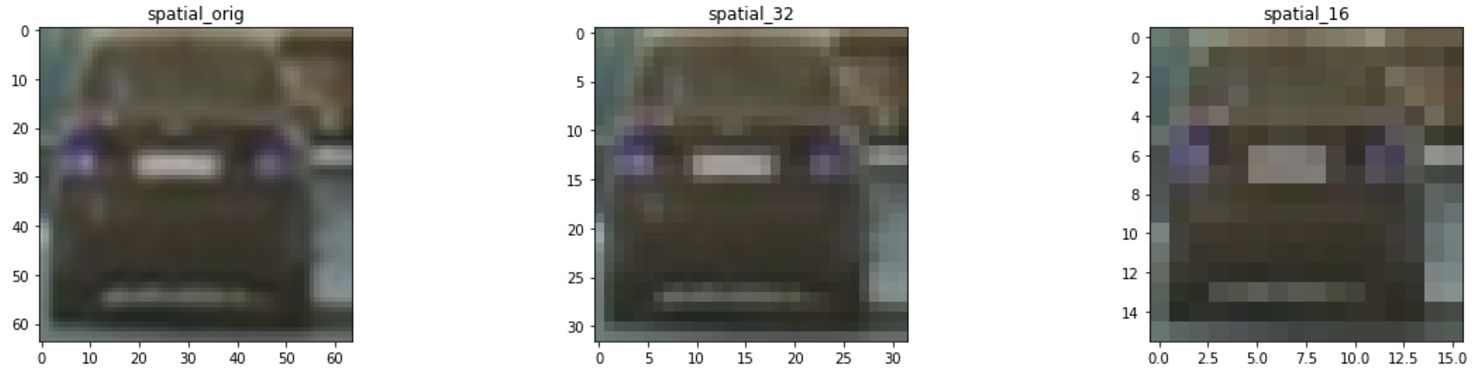
\includegraphics[width=\textwidth]{output_images/feature_spatial.jpg}
        \caption{Spatial features with image sizes of 64, 32 and 16 pixels}
    \label{fig:feature_spatial}
\end{figure}

\subsection{Histogram Features}
The second type of feature is a color histogram. I chose 32 bins per color channel. An example histogram for the color space YCrC is depicted in figure \ref{fig:feature_histogram}.

\begin{figure}[h]
    \centering
    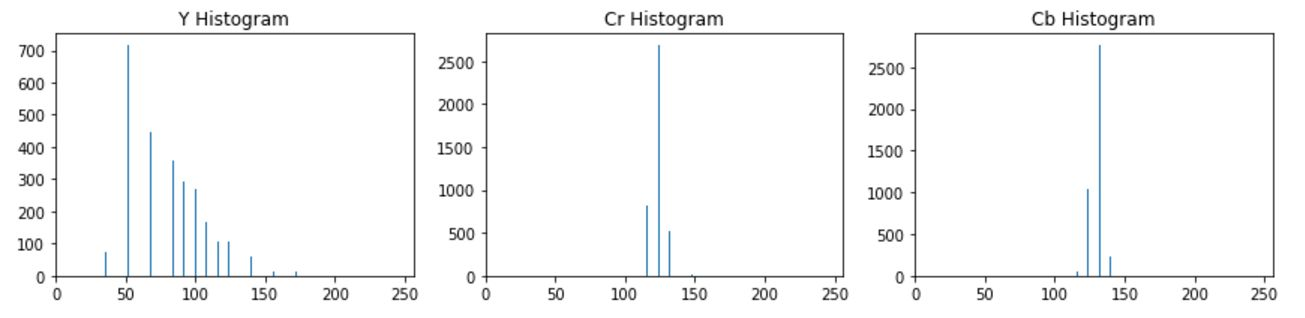
\includegraphics[width=\textwidth]{output_images/feature_histogram.jpg}
        \caption{Histogram features with bin size of 32 for the channels Y, Cr and Cb}
    \label{fig:feature_histogram}
\end{figure}


\subsection{Histogram of Gradients (HOG)}
While the previous two features mostly detect colors, the HOG feature seems to be the best feature to capture the shape of a vehicle. The HOG function has multiple parameters like number of orientations, block and cell size. I explored various combinations, some of them are depicted in figure \ref{fig:feature_hog}. While it is possible to increase classification speed when increasing the number of pixels per cell while maintaining a decent accuracy, I went with a lower number of 8 pxels per cell. I chose 11 orientations, 2 cells per block an all three color channels. This allowed me to achieve a good accuracy as described later.

\begin{figure}[h]
    \centering
    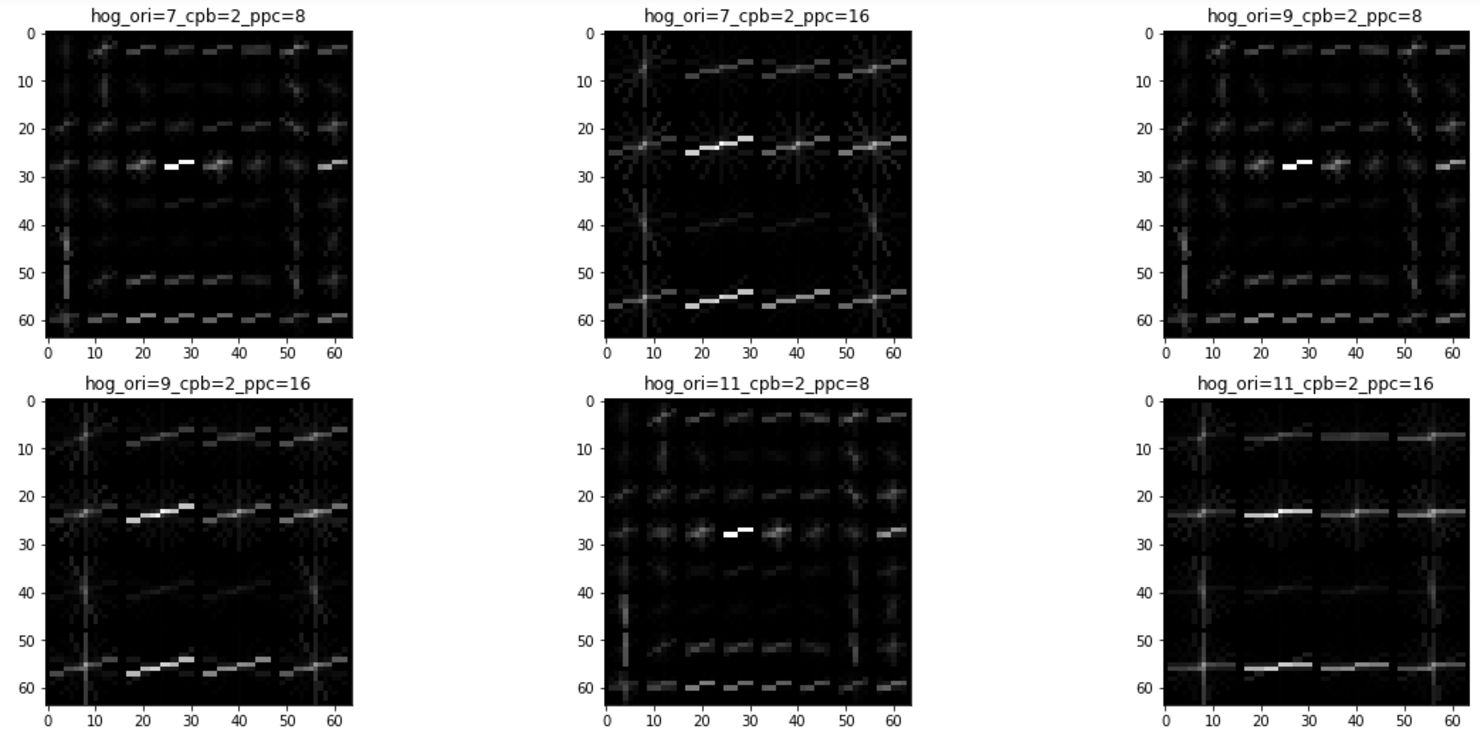
\includegraphics[width=\textwidth]{output_images/feature_hog.jpg}
        \caption{HOG feature images fir different parameters}
    \label{fig:feature_hog}
\end{figure}


\section{Training a classifier}
To train a classifier that can successfully distinguish between vehicles and non-vehicles, I loaded a training set, labeled it, extracted features and then trained a support vector machine with this data.

\subsection{Training Data}
The training data is loaded in cell ``Import Training Data'' of the vehicle\_detection notebook. To achieve a better result in accuracy I added a few vehicle images from the Udacity dataset. That allowed me to have the exact same number of vehicle and non-vehicle images (8968 each).

Aside from that i grouped images that are next to each other as they are extracted from time series images and often show the same car. Using a GroupKFold iterator to split train and test sets will keep images depicting the same car in either training or test set. This reduces overfitting.

After extracting features from the images, the data is normalized using a StandardScaler which is necessary to allow each feature having the same impact on classification. The scaler is saved as it is needed to scale each image later on when classifying it.

\subsection{SVC fitting}
Before fitting the Classifier I used a ExtraTreesClassifier to reduce the number of features by those, that have a small impact on classification. This helps speeding up the training and classification later on. Using this selection model I could reduce the number of features from 9636 features down to 1090 features.

To find the optimal feature generation parameters and evaluate different SVC configurations I used cross\_validation and a GroupKFold iterator. As a trade-off between speed and accuracy I chose a linear SVC as the rbf kernel did not show significant improvement in accuracy. For the linear SVC I used a grid search to find the best C-parameter. As seen in the cell ``Grid search on SVC parameters'' $C=0.001$ achieves the best result. A cross validation in cell ``Train SVC'' shows an accuracy of 0.991 which seems sufficient. 

\section{Vehicle Detection}
To detect vehicles in images and video frames Ia sliding window approach is used to search small patches for cars. The detections are then accumulated and a bounding box is extracted.

\subsection{Sliding Windows}
The sliding windows function is in cell ``Vehicle Detection''. It basically generates a hog for the whole image. This speeds up feature extraction as the HOG features can be reused. The sliding window is moved 2 cells per step in either x- or y-direction until the whole image has been classified. For each windows spatial and histogram features are generated and stacked with the hog features. The feature vector is scaled with the standard scaler and reduced by the selection model. Then the SVC classifies the feature vector. If a vehicle is detection the window is added to a list which is returned in the end (see figure \ref{fig:sliding_windows}.

\begin{figure}[h]
    \centering
    \begin{subfigure}{0.45\textwidth}
        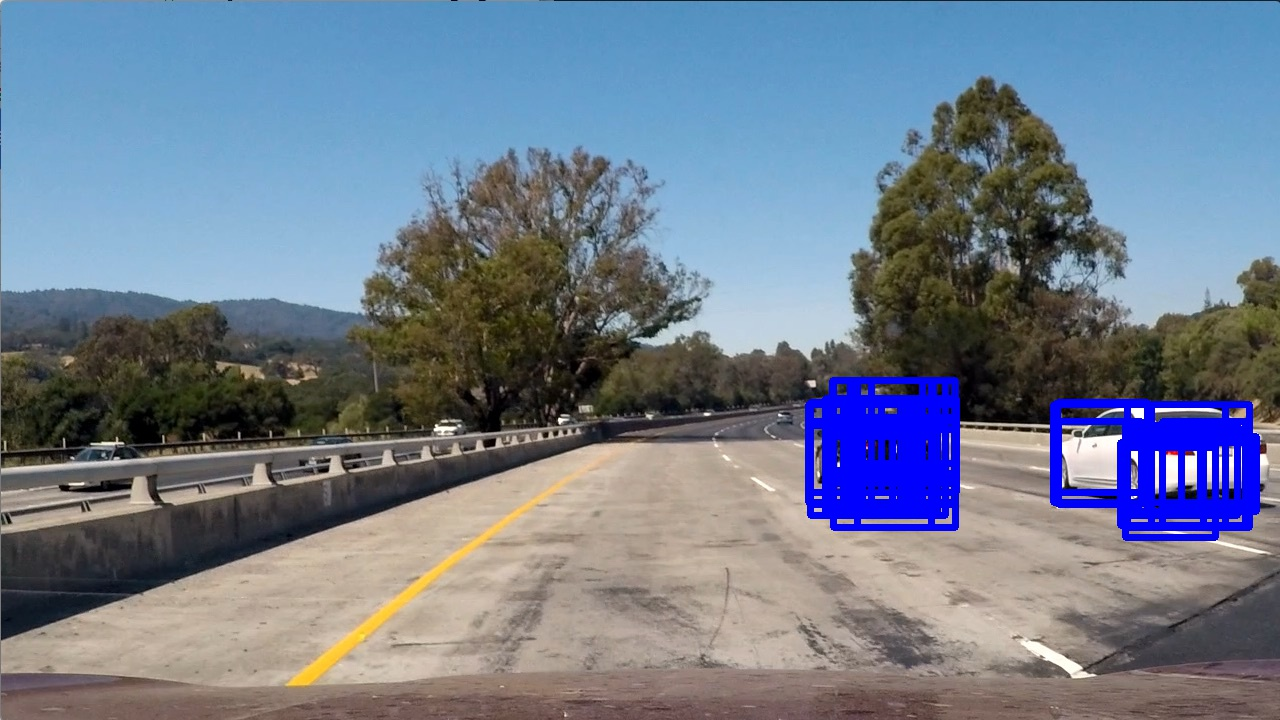
\includegraphics[width=\textwidth]{output_images/test1_bboxes.jpg}
    \end{subfigure}\quad
    \begin{subfigure}{0.45\textwidth}
        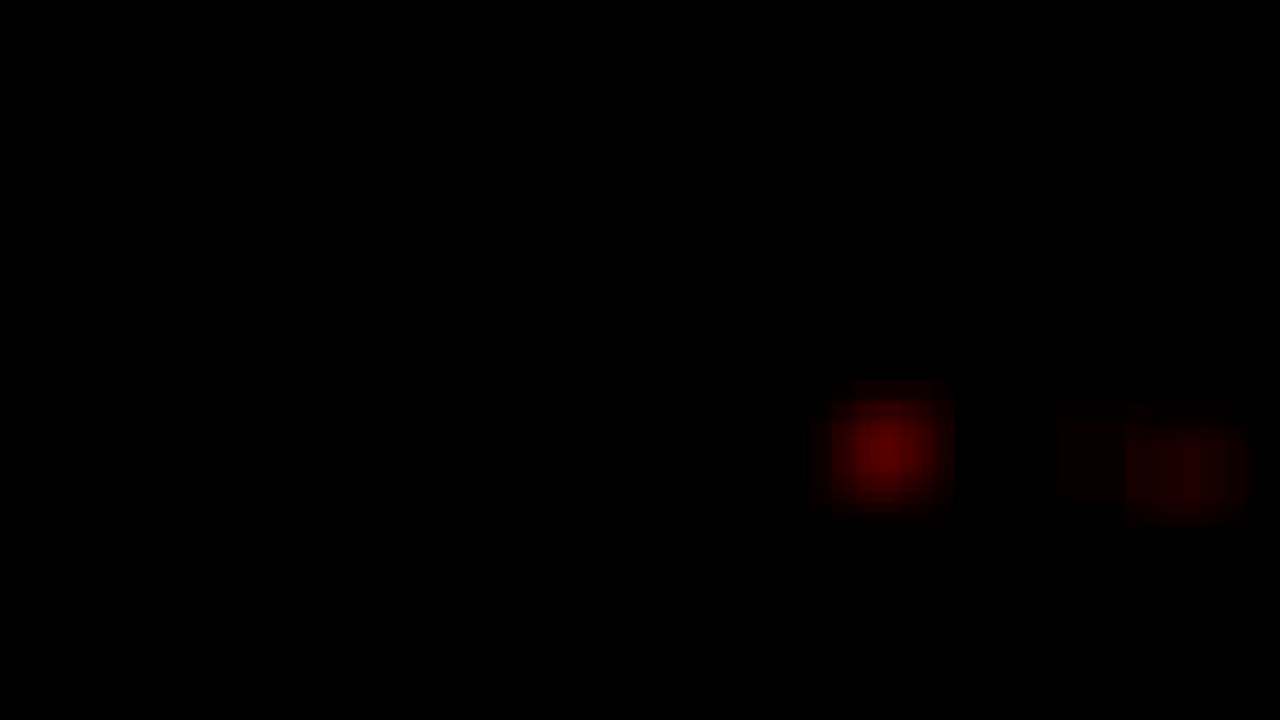
\includegraphics[width=\textwidth]{output_images/test1_heat.jpg}
    \end{subfigure} 
    \caption{Sliding windows on image test01.jpg depicting the overelapping positive detections left and the heat map right.}
    \label{fig:sliding_windows}
\end{figure}

As the cars size in the source image depends on its distance from the camera, the sliding windows approach is done at different image scales for each frame. As this highly increases execution time, the search area for sliding windows is reduced in y-range to cover that part where cars can be expected. A y-range of (380, 660) seemed to work nicely. The area is depicted in figure \ref{fig:y_area}. Three different window sizes are used between 75 and 98 pixels.

\begin{figure}[h]
    \centering
    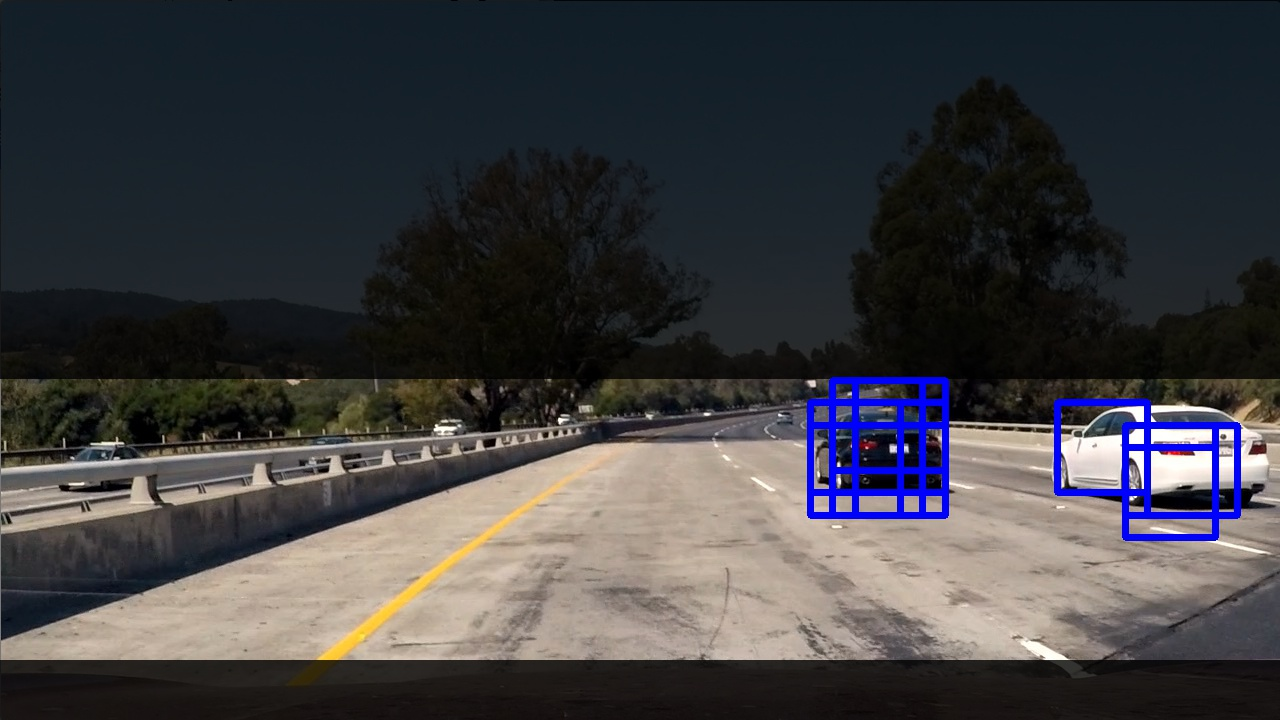
\includegraphics[width=0.7\textwidth]{output_images/test1_range.jpg}
        \caption{Only a subarea of the image where cars can be expected is used for the sliding windows}
    \label{fig:y_area}
\end{figure}

\subsection{Bounding Box Extraction} 
The bounding box of a vehicle is generated by using heat maps. For each window that is detected in the previous step, the window's pixels are incremented in heat map image. The higher a heat value in the resulting image is, the more overlapping windows it had and the more likely it is to be of a vehicle. The heat map is thresholded and labeled using connected components. Afterwards for each component the minimal surrounding rectangle is generated which is the vehicles bounding box.

For videos this step is averaged over several frames. The heat map is accumulated for 5 frames each. This helps reducing false positives. The bounding box that is extracted from the accumulated heat map is also averaged over 5 frames to smooth its size and position. This is being done using the Vehicle class. For each existing vehicle a new bounding box is searched, that covers a large part of the vehicle's current bounding box. if such is found it is added to the vehicles bounding box list replacing the oldest entry. If a vehicle has not seen a matching bounding box for 5 frames it is removed from the list.

\section{Results}
The resulting bounding boxes for the test images can be found in the folder output\_images. For test images 2-5 the results are depicted in figure \ref{fig:test_vehicles}. While there are a few false positives in test02 and test05, the vehicles are classified properly. The false positives can be significantly reduced using averaging as being shown in the project video.

\begin{figure}[h]
    \centering
    \begin{subfigure}{0.45\textwidth}
        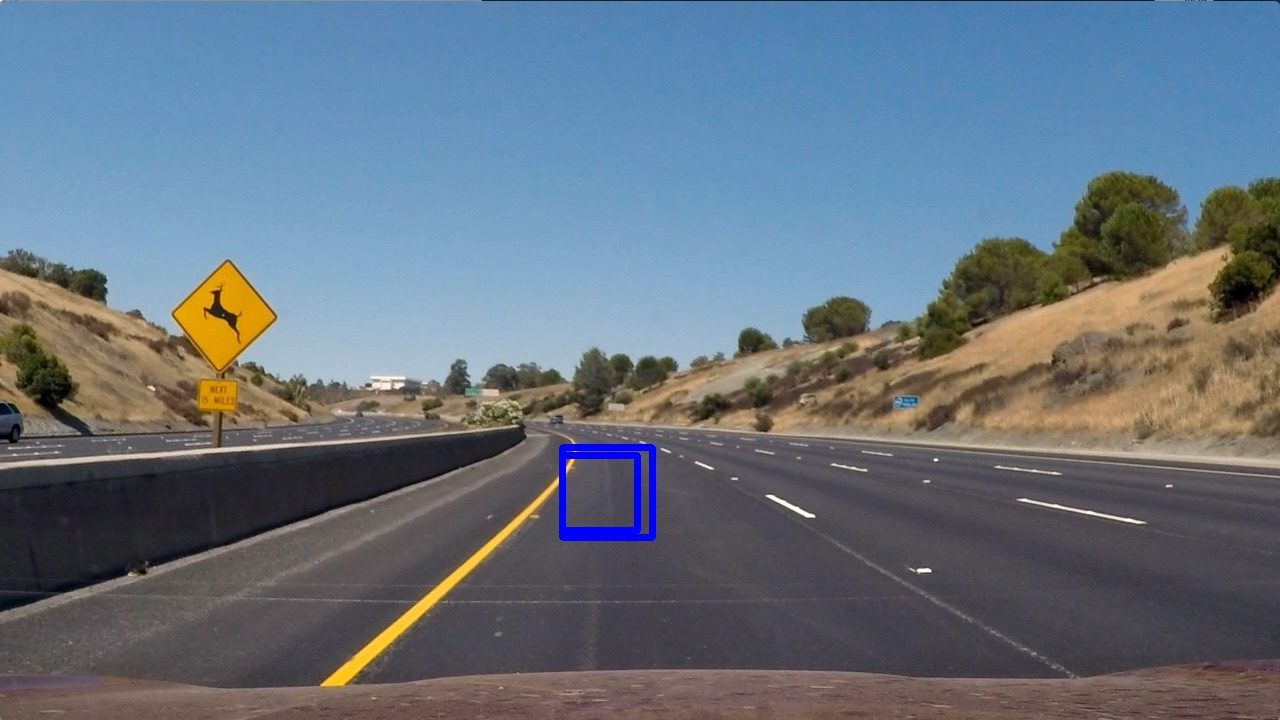
\includegraphics[width=\textwidth]{output_images/test2.jpg}
    \end{subfigure}\quad
    \begin{subfigure}{0.45\textwidth}
        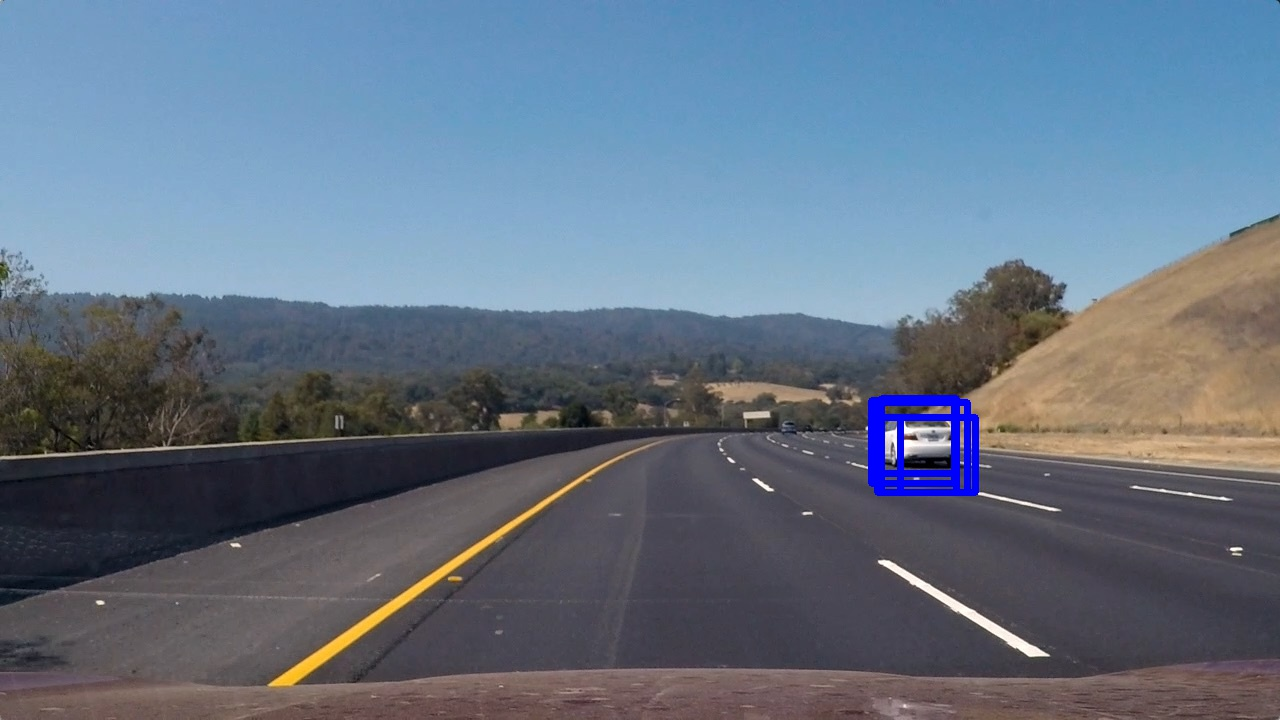
\includegraphics[width=\textwidth]{output_images/test3.jpg}
    \end{subfigure} \\ \medskip
        \begin{subfigure}{0.45\textwidth}
        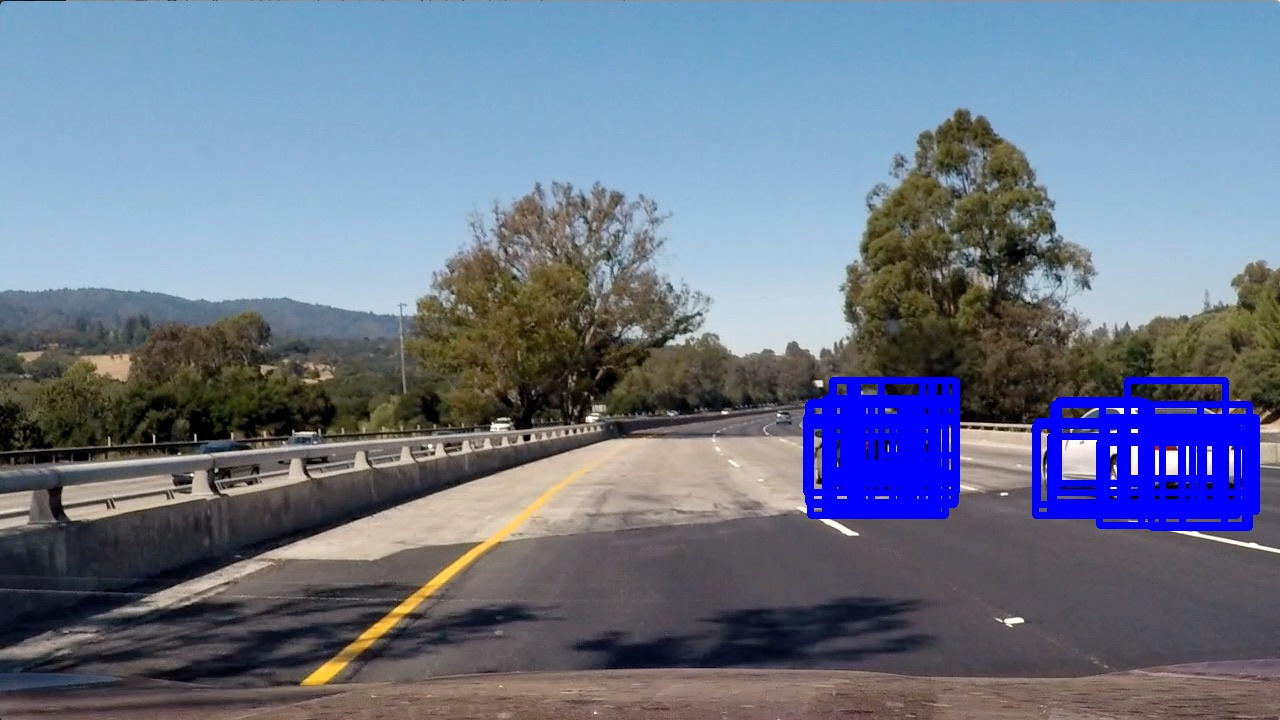
\includegraphics[width=\textwidth]{output_images/test4.jpg}
    \end{subfigure}\quad
    \begin{subfigure}{0.45\textwidth}
        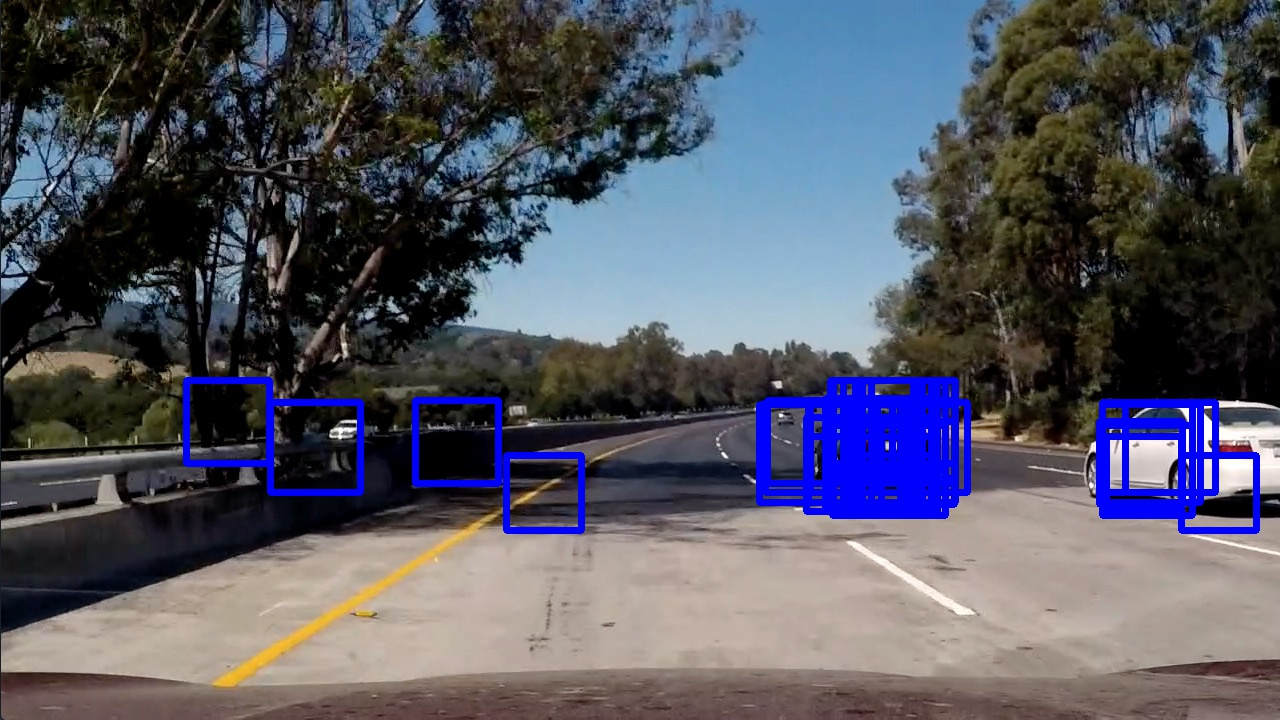
\includegraphics[width=\textwidth]{output_images/test5.jpg}
    \end{subfigure}
    \caption{Vehicle detections for test images 2-5 from top left to bottom right}  
    \label{fig:test_vehicles}
\end{figure}
\section{Discussion}
The classifier seems to be quite accurate on the test set with a score of over 0.99. That being said it does not seem to perform as well on the video frames. I assume a larger dataset for training might achieve better results and reduce false positives.

The sliding window approach works but is relatively slow. I started using more scales by actually checking the maximum and minimum sizes of cars in the video and interpolating 10 scales in-between. As larger windows are less likely to be detected I scaled the added heat values relative to the window size. Further I reduces the search area in y-direction with a decreasing windows size and smaller cars will appear closer to the horizon. The idea seemed plausible and the speed was actually a lot higher but the results weren't pleasing. Interestingly a few small scales seem to work better.

The algorithm for bounding box extraction seems to be quite sensitive to different values for the threshold vehicle matching and they also depend on many other parameters.
%\begin{figure}
%\includegraphics[width=.925\textwidth]{images/preprocess_test02__undistort.jpg}
%\caption{Undistorted test image test02.jpg}
%\label{fig:test02_undistort}
%\end{figure}
%
%\begin{figure}[h]
%    \centering
%    \begin{subfigure}{0.45\textwidth}
%        \includegraphics[width=\textwidth]{images/straight_lines.jpg}
%    \end{subfigure}\quad
%    \begin{subfigure}{0.45\textwidth}
%        \includegraphics[width=\textwidth]{images/straight_lines_warped.jpg}
%    \end{subfigure} 
%    \caption{Bird's view transformation: 4 points on the lane lines were choses that are in shape of a rectangle in world coordinates (assuming the world is flat)}
%    \label{fig:birds_view}
%\end{figure}
%
%
%\begin{figure}[h]
%    \centering
%    \begin{subfigure}{0.45\textwidth}
%        \includegraphics[width=\textwidth]{images/preprocess_test02__hsv_yellow.jpg}
%    \end{subfigure}\quad
%    \begin{subfigure}{0.45\textwidth}
%        \includegraphics[width=\textwidth]{images/preprocess_test02__hsv_white.jpg}
%    \end{subfigure} 
%    \caption{Color thresholds for yellow lines (left) and white lines (right) on test02.jpg.}
%    \label{fig:color_threshold}
%\end{figure}
%
%
%\begin{figure}[h]
%    \centering
%    \begin{subfigure}{0.45\textwidth}
%        \includegraphics[width=\textwidth]{images/preprocess_test02__glx.jpg}
%    \end{subfigure}\quad
%    \begin{subfigure}{0.45\textwidth}
%        \includegraphics[width=\textwidth]{images/preprocess_test02__gsx.jpg}
%    \end{subfigure} 
%    \caption{Gradient thresholds in x-direction ión the L-channe (left) and S-channel (right) on test02.jpg.}
%    \label{fig:gradient_threshold}
%\end{figure}
%
%
%
%\begin{figure}[h]
%    \centering
%    \begin{subfigure}{0.45\textwidth}
%        \includegraphics[width=\textwidth]{images/preprocess_test02__combined-OR.jpg}
%	\caption{or-combined thresholds}
%	\label{fig:threshold_combined}
%    \end{subfigure}\quad
%    \begin{subfigure}{0.45\textwidth}
%        \includegraphics[width=\textwidth]{images/preprocess_test02__warped.jpg}
%    \caption{original image in bird's view}
%    \end{subfigure} 
%    \caption{The combination of all threshold images of the undistorted image test02.jpg in bird's view.}
%    \label{fig:threshold_final}
%\end{figure}
%
%
%\begin{figure}[h]
%    \centering
%    \begin{subfigure}{0.45\textwidth}
%        \includegraphics[width=\textwidth]{images/lane_detection_test02_01.jpg}
%	\caption{Slidng windows}
%	\label{fig:sliding_windows}
%    \end{subfigure}\quad
%    \begin{subfigure}{0.45\textwidth}
%        \includegraphics[width=\textwidth]{images/lane_detection_test02_02.jpg}
%    \caption{polynomial search area}
%    \label{fig:polynomial_search}
%    \end{subfigure} 
%    \caption{The two different search approaches for lane detection. Search areas are marked green, estimated lane position in yellow.}  
%    \label{fig:lane_detection}
%\end{figure}


%\begin{figure}[h]
%    \centering
%    \includegraphics[width=0.925\textwidth]{images/lane_projection_sanity_01.jpg}
%
%    \caption{Red lanes indicate that the lane detection was rejected for this frame..}
%    \label{fig:sanity_check}
%\end{figure} 

\printbibliography
\end{document}
